\documentclass[a0paper,portrait]{baposter}
\usepackage{float}
\usepackage{multicol}
\usepackage{adjustbox}
\usepackage{xcolor}
\usepackage{bm}
\usepackage{enumitem}
\usepackage[ruled,vlined,linesnumbered]{algorithm2e}
\usepackage{amsmath,amsfonts,amssymb,amsthm}
\usepackage[style=authoryear, maxbibnames=99, mincitenames=1, maxcitenames=3, dashed=false, giveninits=true, backend=biber, bibencoding=utf8, uniquename=false, uniquelist=false]{biblatex}
\newtheorem{thm}{Theorem}

\SetAlFnt{\normalsize\sffamily}
\newcommand{\pushline}{\Indp}% Indent
\newcommand{\popline}{\Indm\dosemic}% Undent
\let\oldnl\nl% Store \nl in \oldnl
\newcommand{\nonl}{\renewcommand{\nl}{\let\nl\oldnl}}% Remove line number for one line
\DeclareRobustCommand{\rchi}{{\mathpalette\irchi\relax}}
\newcommand{\irchi}[2]{\raisebox{\depth}{$#1\chi$}} % inner command, used by \rchi
\DeclareMathOperator*{\argmaxA}{arg\,max}
\setlength{\columnsep}{0.6pc}
\defbibenvironment{bibliography}
{\list {}
   {\setlength{\leftmargin}{0.1cm}%
    \setlength{\itemindent}{-0.1cm}%
    \setlength{\itemsep}{\bibitemsep}%
    \setlength{\parsep}{\bibparsep}}}
{\endlist}
{\item}
\addbibresource{biblio.bib}
\graphicspath{{figures/}} % Directory in which figures are stored
\renewcommand*{\bibfont}{\small}

 \definecolor{bordercol}{RGB}{0,43,128}
 \definecolor{headercol1}{RGB}{0,0,204}
 \definecolor{headercol2}{RGB}{77, 166, 255}
 \definecolor{headerfontcol}{RGB}{255,255,255}
 \definecolor{boxcolor}{RGB}{255,255,255}

\begin{document}

\begin{poster}{
    grid=false,
    borderColor=bordercol,
    headerColorOne=headercol1, 
    headerColorTwo=headercol2,
    headerFontColor=headerfontcol, 
    boxColorOne=boxcolor, 
    headershape=roundedright, 
    headerfont=\large\sf\bf, 
    textborder=roundedleft,
    bgColorOne=white,
    background=plain,
    headerborder=open, 
    boxshade=plain,
    headerheight=0.09\textheight,
    colspacing=0.3em,
    textfont=\normalsize\sffamily,
    boxpadding=0.3em,
    columns=4
}
{
\includegraphics[scale=0.25]{QUT_logo.jpg}}
%{\bf \huge {A model robust subsampling approach for Generalised Linear Models in big data settings} }
{\bf \huge {A model robust design approach for optimally sub-sampling big data} }
{\vspace{0.3em} \smaller Amalan Mahendran$^{1,2}$, Helen Thompson$^{1,2}$, James M. McGree$^{1,2}$ \\
\normalsize{$^1$\it {School of Mathematical Sciences, Queensland University of Technology}} \\ $^2$\it{Centre for Data Science, Queensland University of Technology} }
{
\includegraphics[scale=0.1]{qr-code_Article_Arxiv.eps}}

% INTRODUCTION
\headerbox{1. Introduction}{name=introduction,column=0,span=2,boxheaderheight=1.55em}{
Subsampling methods have been proposed as computationally efficient approaches to analyse big data. 
Here, we consider sampling big data $F_N=(\bm{X}_0,\bm{y})$, with data matrix $\bm{X}_0=({\bm{x}_0}_1,\ldots,{\bm{x}_0}_N)^T \in R^{N \times p}$ and response vector $\bm{y}=(y_1,\ldots,y_N)^T$, based on subsampling probabilities $\phi$, where $\phi$ is based on an optimality criterion e.g. A-optimality \parencite{ai2021optimal}. 
However, a key limitation of this approach is that $\phi$ depends on an assumed model through the optimality criterion, and such a model may be difficult to specify in practice. 
To overcome this limitation, we propose to consider a set of models and a model averaging approach for determining $\phi$.
%The computational challenge of big data analysis can be overcome by, instead, analysing an optimal subsample of the big data. 
%We consider randomly sampling big data set $F_N=(\bm{X}_0,\bm{y})$, with data matrix $\bm{X}_0=({\bm{x}_0}_1,\ldots,{\bm{x}_0}_N)^T \in R^{N \times p}$ and response vector $\bm{y}=(y_1,\ldots,y_N)^T$, based on subsampling probabilities $\phi$. 
%Here, $\phi$ depends on the specific statistical model and criteria of optimality for the subsample, e.g., $A$-optimal parameter estimation in Generalised Linear Models \parencite{ai2021optimal}. 
%A key limitation is that the assumed statistical model may not appropriately describe the big data. Rather than selecting a single assumed best candidate model, we propose considering a set of models and a model averaging approach in determining $\phi$.
}

% Background
\headerbox{2. Generalised Linear Models (GLMs) }{name=background,span=2,column=0,boxheaderheight=1.55em,below=introduction}{
A GLM is defined via three components:  
    \begin{itemize}[itemsep=-3pt,topsep=-3pt,leftmargin=*]
        \item distribution of $\bm{y}$, such that $f(y;\omega,\gamma)=\exp{\left(\frac{y\omega - \psi(\omega)}{a(\gamma)} + b(y,\gamma) \right)}$, for some functions $\psi(.), a(.)$ and $b(.)$, natural parameter $\omega$ and dispersion $\gamma$;
        \item linear predictor $\bm{\eta}=\bm{X}\bm{\theta}$, where $\bm{\theta}=(\theta_1,\ldots,\theta_{p+t})^T$ is the parameter vector and $\bm{X}=h(\bm{X}_0) \in R^{N \times (p+t)}$ for some function $h(.)$, i.e., columns may be appended to $\bm{X}_0$ in big data set $F_N$ corresponding to an intercept and/or higher-order terms to create $\bm{X}$; and
        \item link function $g(.)$, such that $g(\bm{\mu})=\bm{\eta}$ for $\bm{\mu}=E(\bm{y})$.
    \end{itemize}
    %For logistic regression, $\bm{y} \sim \mbox{Bin}(n,\bm{\pi})$ and $g(.)$ is the logit link function $g(\bm{\pi})=\log(\bm{\pi}/(1-\bm{\pi}))$ such that $g(\bm{\pi})=\bm{X}\bm{\theta}$.
}

% General subsampling algorithm
\headerbox{3. General subsampling algorithm}{name=GSA,column=0,span=2, below=background, boxheaderheight=1.55em}{
Algorithm~\ref{Algo:GenSam} is a subsampling algorithm for GLMs, where $\bm\theta$ is estimated using a weighted log-likelihood with weights $\frac{1}{\phi}$.

    \begin{algorithm}[H]
    \SetAlgoLined
        \textbf{Sampling:} Assign $\phi_i$ to $\{\bm{x}_i,y_i\}$, for $i=1,...,N$, $\phi_i \in (0,1)$, $\sum_{i=1}^{N} \phi_i=1$, and draw a subsample of size $r$ from $(\bm{X},\bm{y},\bm{\phi})$ with replacement to yield $S = \{\bm{x}_l^*,y_l^*,\phi_l^*\}_{l=1}^r = (\bm{X}^*,\bm{y}^*,\bm{\phi}^*)$. \\
        \textbf{Estimation:} Based on $S$, find
        $\tilde{\bm{\theta}} = \argmaxA_{\bm{\theta}} \log{L(\bm{\theta}|\bm{X}^*,\bm{y}^*,\bm{\phi}^*)} \equiv \argmaxA_{\bm{\theta}} \frac{1}{r} \sum_{l=1}^{r} \frac{y^*_l u(\bm{\theta}^T\bm{x}^*_l) - \psi(u(\bm{\theta}^T\bm{x}^*_l))}{\phi^*_l}.$ \textbf{Output:} $\tilde{\bm{\theta}}$ and $S$.
    \caption{General subsampling algorithm \textcite{ai2021optimal}} \label{Algo:GenSam}
    \end{algorithm} 
%The $\phi$ values are assigned based on %asymptotic properties 
To determine the values of $\phi$, %of $\bm{\tilde{\theta}}$. 
\textcite{ai2021optimal} considered the $A$-optimality criterion, corresponding to minimisation of the asymptotic mean squared error of $\tilde{\bm{\theta}}$ ($\mbox{tr}(\bm{V})$), to obtain the subsampling probabilities:
        \begin{equation}\label{Eq:1}
            \phi_i = \frac{|y_i - \dot{\psi}(u(\hat{\bm{\theta}}^T_{MLE}\bm{x}_i))|\, ||\bm{J}^{-1}_{\bm{X}} \dot{u}(\hat{\bm{\theta}}^T_{MLE}\bm{x}_i)\bm{x}_i ||}{\sum_{j=1}^{N} |y_j - \dot{\psi}(u(\hat{\bm{\theta}}^T_{MLE}\bm{x}_j))|\, ||\bm{J}^{-1}_{\bm{X}} \dot{u}(\hat{\bm{\theta}}^T_{MLE}\bm{x}_j)\bm{x}_j ||},    
        \end{equation}
        
where $\hat{\bm{\theta}}_{MLE}$ is an estimate of $\bm{\theta}$ based on the whole big data set and $\bm{J_X}$ is the observed information matrix. 
As $\bm{\phi}$ depends on $\hat{\bm{\theta}}_{MLE}$, a two stage subsampling strategy was proposed where an initial subsample was used to provide an estimate of $\hat{\bm{\theta}}_{MLE}$. 
%$\phi^{mMSE}$ is conditional on the assumption of a model being appropriate to describe the big data, which is a potential limitation as proposing such a model in practice could be difficult, and there could be a variety of models that appropriately describe the data.
}

% Model robust optimal subsampling method
\headerbox{4. Model robust optimal subsampling method}{name=MROS, below=GSA,span=2, column=0,boxheaderheight=1.4em}{
Following \textcite{ai2021optimal}, $\phi$ depends on a model that is assumed to appropriately describe the big data.
%\textcite{ai2021optimal} calculate $\bm{\phi}$ under the assumption that the model is appropriate to describe the big data. 
Unfortunately, proposing such a model can be difficult in practice, and there may be a variety of models that appropriately describe the data.
%Rather than assuming a single model,
To overcome this, we consider a set of $Q$ models that encapsulate a variety of scenarios that may be observed within the big data. 
For each model, we define model probabilities $\alpha_q$ for $q=1,\ldots,Q$ such that $\sum_{q=1}^Q\alpha_q=1$, which represents our {\it a priori} belief about the appropriateness of each model. The subsampling probabilities are then given by \textbf{Theorem 1}.

\begin{thm}
For a set of $Q$ models with model probability $\alpha_q$ for the $q$-th model, $q=1,\ldots Q$, if the subsampling probabilities are selected as follows: 
\begin{center}
$\phi_i = \sum_{q=1}^{Q} \alpha_q \phi_{qi},$
\end{center}
where $\sum_{q=1}^{Q} \alpha_q = 1$ and $\phi_{qi}$ is given by Eq.~\eqref{Eq:1} for the $q$-th model, then $\sum_{q=1}^{Q} \alpha_q \mbox{tr}(\bm{V}_q)$ attains its minimum -- $\mbox{tr}(\bm{V}_q)$ is the asymptotic mean squared error of $\tilde{\bm{\theta}}$ corresponding to model $q$.
\end{thm}
}

% Simulation Study
\headerbox{5. I) Setup of simulation study - Logistic regression}{name=SimStudy,span=2,column=0,below=MROS,boxheaderheight=1.55em}{
Compare random sampling (RS), optimal subsampling (OS) and model robust optimal subsampling (MROS) for models in Table~1. Use $\alpha_q=1/4$, $N=10000$, $M=1000$ simulations and subsample sizes $r=100,200,\ldots,1400$.
\vspace{-0.35em}
        \begin{table}[H]
            \centering %\small{
            \begin{tabular}{l} \hline
            \textbf{Table 1:} Model set for $F_N$ \\ \hline
            $-2 + 1.5 \bm{x}_1 + 0.3 \bm{x}_2$ \\
            $-2 + 1.7 \bm{x}_1 - 1.2 \bm{x}_2 + 0.2 \bm{x}^2_1$ \\ 
            $-2 - 1.3 \bm{x}_1 + 1.9 \bm{x}_2 + 0.9 \bm{x}^2_2$ \\ 
            $-2 + 1.9 \bm{x}_1 + 1.9 \bm{x}_2 + 0.9 \bm{x}^2_1 + 0.7 \bm{x}^2_2$ \\ \hline
        \end{tabular} %}
        \end{table} 
}
\headerbox{5. II) Simulation study - methodology and results}{name=SimStudy2,span=2,column=2,boxheaderheight=1.55em}{
    \begin{itemize}[leftmargin=*,itemsep=-3pt,topsep=-3pt]
            \item For each model, $F_{N}$ was constructed by using an exponential distribution to generate covariates ($x_1,x_2$) and a logistic regression model for the corresponding response ($y$). The performance of the sampling methods was then compared for each $F_{N}$ through evaluating six scenarios: 
            \setlist[itemize]{align=left}
            \begin{itemize}[labelwidth=2.5em, leftmargin=3em, rightmargin=1em, itemsep=-2pt]
                \item[1.] RS to estimate parameters of data generating model;
                \item[2.] OS under data generating model;
                \item[3 -- 5.] OS under alternative models i.e., to estimate parameters of data generating model using samples obtained from alternative model;
                \item[6.] MROS to estimate  parameters of data generating model.
            \end{itemize}
            \item Simulated Mean Squared Error (SMSE) was used to compare each approach as follows: $SMSE(\bm{\theta}) = \frac{1}{M}{\sum_{m=1}^{M} \sum_{n=1}^{p+t} (\tilde{\theta}_{nm} - \theta_n)^2 },$ where $\theta_n$ is the $n$-th underlying parameter of the data generating model and $\tilde{\theta}_{nm}$ is the estimate of this parameter from the $m$-th simulation.
            \item Under OS, the data generating model (red) is typically preferred within the model set (smallest SMSE), as it is the case where the appropriate data generating model was correctly assumed to describe the big data (Fig.~\ref{Fig:1}).
            \item Increases in the SMSE are observed when the incorrect model (pink) is considered for OS compared to the data generating model (red). The proposed model robust approach (green) performs similarly to the OS approach (red). 
        \end{itemize}
        \begin{figure}[H]
            \centering
            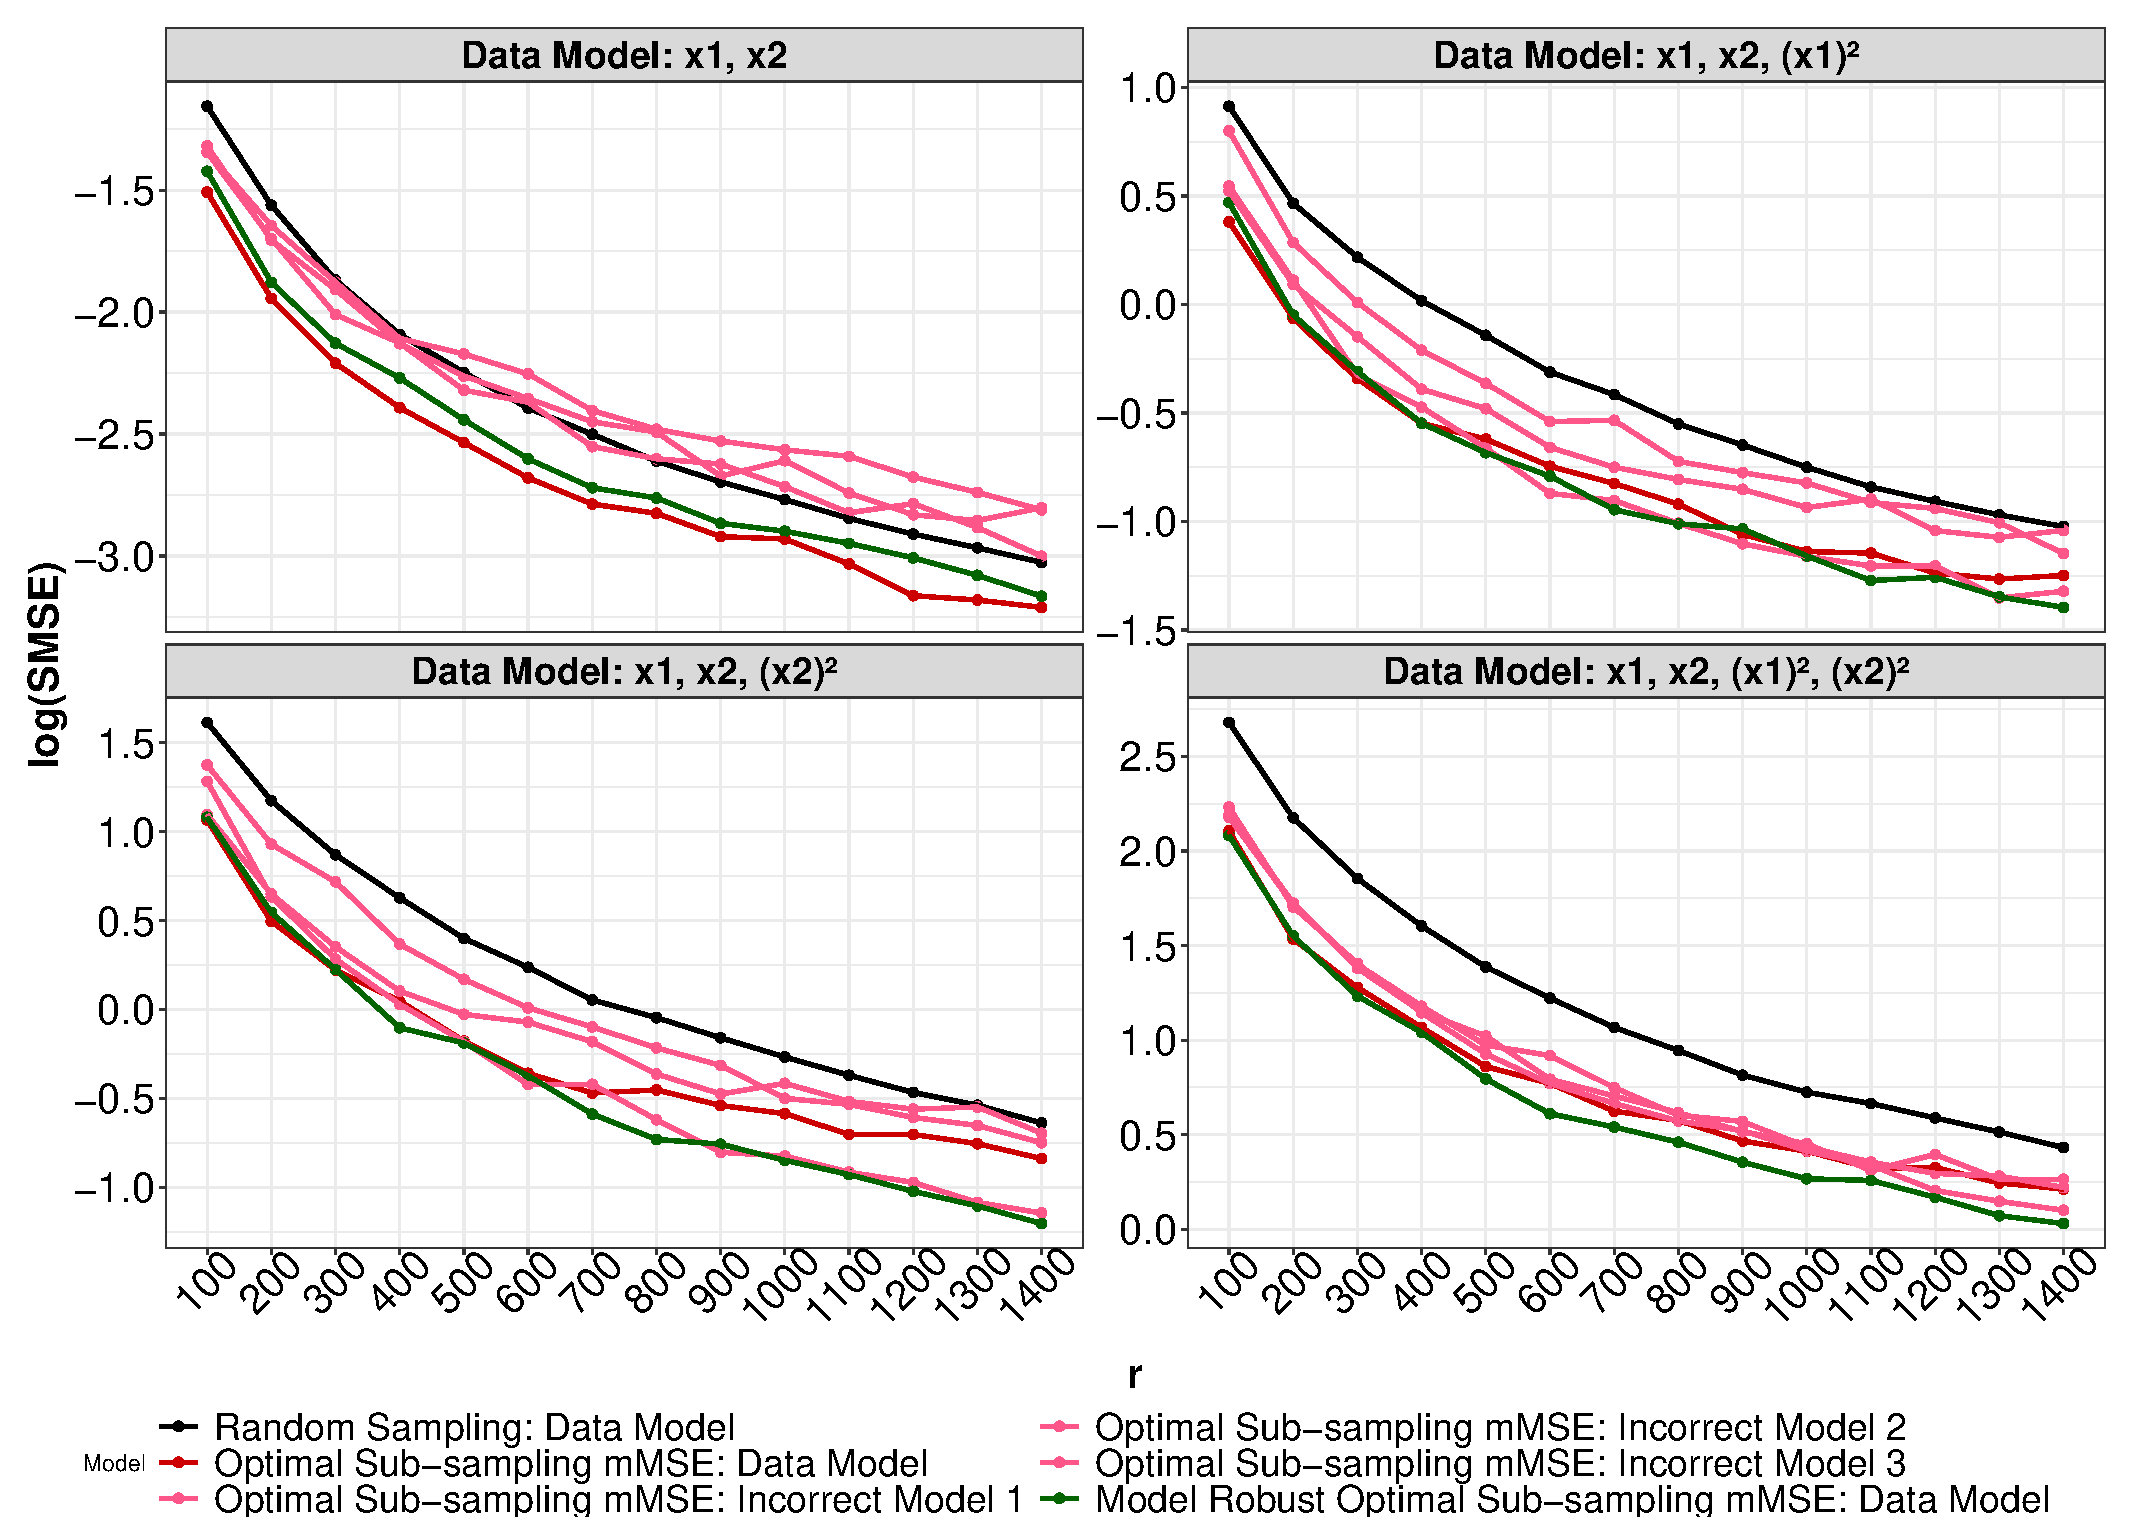
\includegraphics[width=\textwidth,keepaspectratio]{Poster_SMSE_LR_TV_Exp_mMSE.eps}\vspace{-0.3cm}
            \caption{\smaller{Logarithm of SMSE (smaller is better) for the subsampling methods for the logistic regression model.}}\label{Fig:1}
        \end{figure}
}

% Real World Applications
\headerbox{6. Real world application}{name=application,span=2,column=2,below=SimStudy2,boxheaderheight=1.55em}{
    \begin{multicols}{2}
        \begin{itemize}[leftmargin=*,itemsep=-3pt,topsep=-3pt]
            \item ``Skin segmentation'' data, classify $N=245,057$ face images (out of which $50,859$ are skin samples and $194,198$ are non-skin samples) based on RGB (R-red, G-green, B-blue) values of randomly sampled pixels.
            \item $Q=8$ models, includes the main effects model, with intercept, and all possible combinations of quadratic terms for continuous covariates. SMSE under each subsampling method was evaluated for various $r$ and $M=1000$ simulations as $SSMSE(\hat{\bm{\theta}}) = \sum_{q=1}^{Q} SMSE_q(\hat{\bm{\theta}})$.
            \item MROS (green) consistently outperforms OS (red) and RS (black) (Fig.~\ref{Fig:2}).\vspace{-0.35cm}
        \end{itemize}
        \begin{figure}[H]
        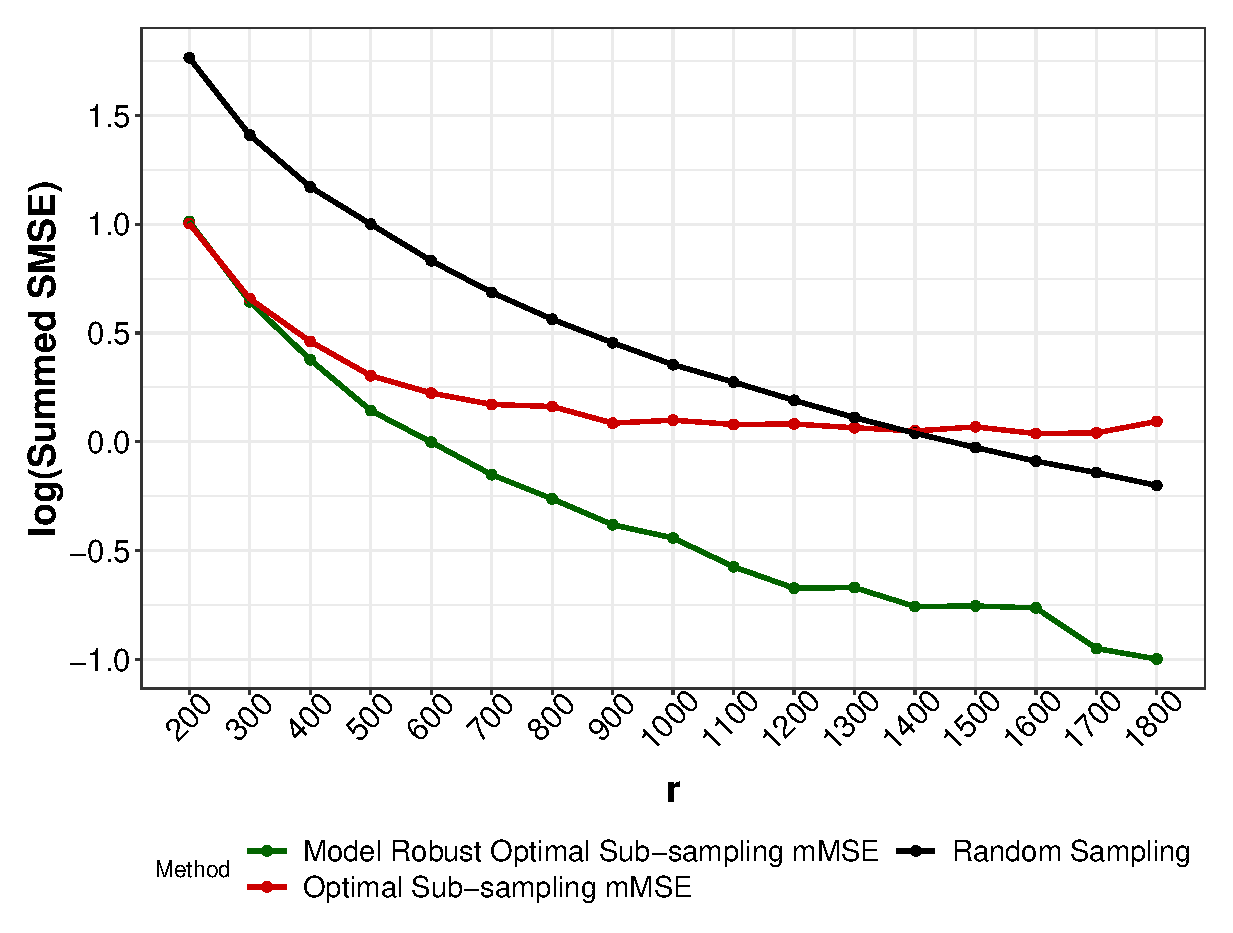
\includegraphics[keepaspectratio,scale=0.28]{Poster_RWA_LR_SkinData.eps} \vspace{-0.4cm}
        \centering
        \caption{\smaller{Logarithm of summed SMSE over the available models for logistic regression applied on the ``Skin segmentation'' data.}}\label{Fig:2}\vspace{2em}
        \end{figure}
    \end{multicols}
}

% CONCLUSION
\headerbox{7. Conclusion}{name=conclusion,column=2,below=application,span=2,boxheaderheight=1.55em}{
Our MROS approach, with supporting theoretical results, performs better than OS and RS for various subsample sizes.
Future work is to extend our approach for a flexible set of models for example Generalised Additive Models or the inclusion of a discrepancy term in the linear predictor.
}

% REFERENCES
\headerbox{\normalsize References}{name=references,span=2, column=2,below=conclusion,boxheaderheight=1.3em}{
\renewcommand{\section}[2]{\vskip 0.05em} % Get rid of the default "References" section title
\nocite{*}
\printbibliography}

\end{poster}

\end{document}